\section{Status Register}

\bilingal{%
状态寄存器中主要保存了因执行最近一次 ALU 运算而产生的结果信息。这些信息用于控制
程序执行流程。状态寄存器是在 ALU 操作完全结束后更新,这样就可以省去了使用单独的
比较指令,可以带来更加紧凑高效的代码实现。状态寄存器的值在响应中断和从中断中退出
时并不会自动保存和恢复,这需要软件去实现%
}{%
The Status Register contains information about the result of the most recently
executed arithmetic instructions. This information can be used for control
program execution flow. Status Register is updated after all ALU operations,
this will in many cases remove the need for using the dedicated compare
instructions, resulting in faster and more compact code. The Status Register is
not automatically stored when entering an interrupt routine and restored when
returning from an interrupt. This must be handled by software.%
}

\begin{table}[b]
\caption{SREG Definitions.\label{tab:sreg-definitions}}
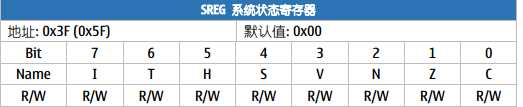
\includegraphics[width=\columnwidth]{Images/f-005}
\end{table}

\begin{description}
\item[(0) C]
\bilingal{%
进位标志,表示算术或逻辑操作导致了进位,具体请参考指令描述
}{%
The Carry Flag C indicates a carry in an arithmetic or logic operation. See the
Section~\myref{sec:instruction-set} for detailed information.%
}

\item[(1) Z]
\bilingal{%
零标志,表示算术或逻辑运算的结果为零,请参考指令描述部分
}{%
The Zero Flag Z indicates a zero resultin an arithmetic or logic operation. See the
“Instruction Set Description” for detailed information.%
}

\item[(2) N]
\bilingal{%
负标志,表示算术或逻辑运算产生了一个负数,请参考指令描述部分
}{%
The Negative Flag N indicates a negative result in an arithmetic or logic operation.
See the “Instruction Set Description” for detailed information%
}

\item[(3) V]
\bilingal{%
溢出标志,表示二进制补码运算结果产生溢出,请参考指令描述部分
}{%
The Two’s Complement Overflow Flag V supports two’s complement arithmetic.
See the “Instruction Set Description” for detailed information.
}

\item[(4) S]
\bilingal{%
符号位,等效于 N 与 V 的异或运算结果,具体请参考指令描述部分
}{%
The S-bit is always an exclusive or between the Negative Flag N and the Two’s
Complement Overflow Flag V. See the “Instruction Set Description” for detailed
information%
}

\item[(5) H]
\bilingal{%
半进位标志,在 BCD 运算中有用,表示字节运算产生了的半进位
}{%
Half Carry Flag :The Half Carry Flag H indicates a Half Carry in some arithmetic
operations. Half Carry Is useful in BCD arithmetic.%
}

\item[(6) T]
\bilingal{%
临时位,位复制(BLD)和位存储(BST)指令中使用,T 位将作为一个临时的存储位,用于临时
存放通用寄存器中的某一位的值。具体请参考指令描述部分%
}{%
Bit Temporary Copy Storage: The Bit Copy instructions BLD (Bit Load) and BST
(Bit Store) use the T-bit as source or destination for the operated bit temporarily. A
bit from a register in the Register File can be copied into T. See the “Instruction
Set Description” for detailed information
}

\item[(7) I]
\bilingal{%
全局中断使能位,必须设置此位为 1 才能使能内核响应中断事件。不同的中断源是由独立
的控制位控制。全局中断使能位是控制中断信号进入内核的最后一道屏障。 I 位在内核响
应中断向量后由硬件自动清除,在执行中断返回指令(RETI)后自动置位。I 位也可以使用
SEI 和 CLI 指令改变,请参考指令描述部分%
}{%
The Global Interrupt Enable bit must be set as 1 for the interrupts to be
enabled.The individual interrupt enable control is then performed in separate
control registers. If the Global Interrupt Enable Register is cleared, none of
the interrupts are enabled independent of the individual interrupt enable
settings. The I-bit is cleared by hardware after an interrupt has occurred, and
is set by the RETI instruction to enable subsequent interrupts. The I-bit can
also be set and cleared by the application with the SEI and CLI instructions, as
described in the instruction set reference.%
}
\end{description}